%!TEX program = xelatex
\documentclass[10pt,mathserif]{beamer}%,aspectratio=169 %画面比例16:9%
\setbeamercovered{invisible}

\usepackage{xeCJK}
\setCJKmainfont{Noto Sans CJK SC}
\setmonofont{Noto Sans Mono}

\usepackage{listings}
\lstset{
basicstyle=\small\ttfamily,
keywordstyle=\color{blue},
numbers=left,
numberstyle=\tiny,
frame=leftline,
tabsize=4
}

\lstdefinestyle{term}
{basicstyle=\ttfamily, numbers=none, frame=single, breaklines=true,
moredelim={[is][keywordstyle]{@@}{@@}}}

\usetheme[
% sidebar, % 会在每页左侧加上导航栏,参考 The AAU Sidebar Beamer Theme 设置
 xdblue, % 不选会默认西电红色调,选上会将主题设置为西电蓝色调
% english % 选上,会将图表等标题还原回英文标题
 ]{XDUstyle}

\usepackage{ulem}

\title{程序调试}
\subtitle{Debugging}
\institute[西安电子科技大学\\程序设计竞赛实训基地]{西安电子科技大学空间科学与技术学院} % 中括号部分为导航栏底所用尽可能精简
\author{席若尧}
\date{2019 年 7 月 8 日}% 时间可自行设置
	
\begin{document}%
{\xdbg \frame[plain,noframenumbering]{\titlepage}}%首页标题页

\begin{frame}{注意事项}
	\begin{itemize}
		\item 本课程相关资料课后会下发/公开。
		\item 由于主讲人比较菜,如果讲错了请及时指出。
	\end{itemize}
\end{frame}

\begin{frame}{自我介绍}
	\begin{itemize}
		\item 空间院 2019 级博士\tiny(硕士毕不了业只能继续苟着的屑)
			\normalsize
		\item 曾获 2015 年省赛冠军\tiny(陕西省)
			\normalsize
		\item 邀请赛 1 铜 2 银,区域赛 3 铜 3 银\tiny(没有金牌的退役狗)
			\normalsize
		\item Codeforces: \textcolor[rgb]{1,0.549,0}{orz\_liuwei}\tiny(走狗屎运上了分就赶紧换号了)
			\normalsize
	\end{itemize}
\end{frame}

\part{引言}

\begin{frame}{BUG!}
	在比赛和训练中,往往出现以下现象:
	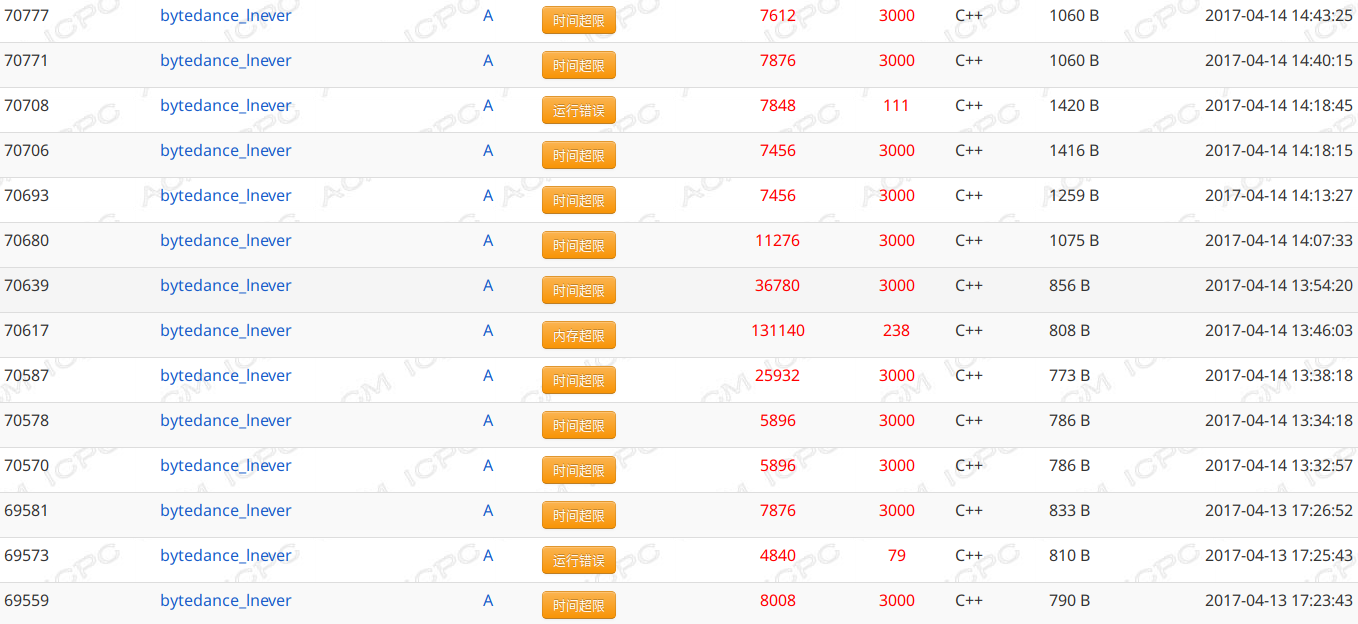
\includegraphics[width=\textwidth]{img/bug.png}
\end{frame}

\begin{frame}{BUG!}
	在比赛和训练中,往往出现以下现象:
	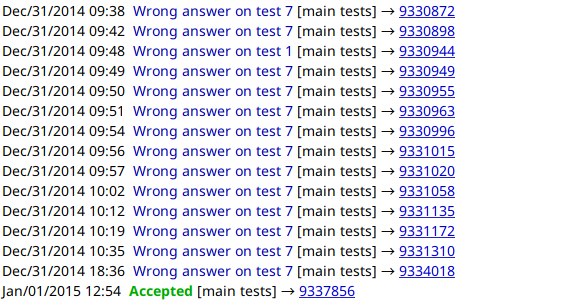
\includegraphics[width=\textwidth]{img/bug1.png}
\end{frame}

\begin{frame}{然后就自闭了}
	\center
	
\includegraphics[width=.6\textwidth]{img/wa.png}
\end{frame}

\begin{frame}{一切都是调试}
	\begin{itemize}
		\item 写程序
			\begin{itemize}
				\item 软件开发中一半以上时间用于测试和调试
			\end{itemize}
		\item 做电路
		\item 复习考试
		\item 物理学(?)
	\end{itemize}
\end{frame}

\begin{frame}{技术归零}
	根据中国航天科技集团公司 Q/QJA 10-2002 标准,质量问题技术归零要做到:
	\begin{itemize}
		\item 定位准确
		\item 机理清楚
		\item 问题复现
		\item 措施有效
		\item 举一反三
	\end{itemize}
	\tiny 除了技术归零以外还有管理归零:
	过程清楚、责任明确、措施落实、严肃处理、完善规章
\end{frame}

\begin{frame}{Bug 分类}
	\begin{itemize}
		\item 语法错误?
		\item 语义错误?
	\end{itemize}
\end{frame}

\begin{frame}[fragile]{Bug 分类}
	\begin{itemize}
		\item 语法错误 -> CE \\
			例如:\lstinline!(1+x;!
		\item 语义错误
			\begin{itemize}
				\item 违反约束条件 -> CE \\
					例如:\lstinline[language=C++]!int a; char a;!
				\item 违反其他语义规则 -> \textbf{未定义的} \\
					例如:\lstinline[language=C++]!int x[2]; x + 3;!
				\item “纯粹”的逻辑错误 -> WA, TLE, MLE, OLE \\
					例如:算法假了
			\end{itemize}
	\end{itemize}
\end{frame}

\begin{frame}{关于未定义行为}
	某些人总是无视语言标准尝试使用各种未定义行为,
	然后到处说“这程序在我的电脑上能工作,为什么交上去就错?”
	对此,Roger Miller 讽刺道:
	\begin{itemize}
		\item 有人曾经告诉我,在打篮球的时候,你不能持球跑动。
			我买了个篮球然后试了一下,发现跑得很好。
			这说明那人根本不懂篮球。
	\end{itemize}
	\pause
	\center
	
\includegraphics[width=.5\textwidth]{img/cxk.jpg}
\end{frame}

\part{程序设计竞赛中常见的编程错误}

\section{栈溢出}
\begin{frame}{什么是栈溢出}
	\begin{itemize}
		\item 函数调用的过程中会把一些数据(返回地址,局部变量,部分参数)
			放入系统的栈空间中,调用结束后再弹出。
			\tiny(简老师 7 月 2 日讲了)
			\normalsize
		\item 为了更灵活地为堆和共享库分配内存,Linux 默认将栈空间限制在 8MB。
		\item 如果栈的大小越过 8MB,内核会发送 \lstinline!SIGSEGV!
			信号杀死进程
		\item Windows 默认栈空间限制为 1MB
	\end{itemize}
\end{frame}

\begin{frame}{栈溢出的表现}
	\begin{itemize}
		\item Runtime Error
		\item 段错误
		\item segmentation fault (core dumped)
	\end{itemize}
\end{frame}

\begin{frame}{预防和排查}
	\begin{itemize}
		\item 绝对不要写死递归
		\item \sout{ICPC 区域赛会调整系统栈空间限制,因此可以随便使用栈(除非
			MLE)}
			\begin{itemize}
				\item Codeforces 调整到了 256MB
				\item 然而大多数在线评测系统都没有调整
			\end{itemize}
		\item 可以将本机调成分配尽量大的栈空间:
			\lstinline|ulimit -s unlimited|
			\begin{itemize}
				\item 只对当前终端开出来的进程有效
				\item 这会导致死递归难以排查,甚至卡死系统,
					可以选择折中地把栈调大一点:
					\lstinline|ulimit -s 131072| (单位 KB)
			\end{itemize}
		\item 不要将巨大的数组或结构体声明为自动局部变量或按值传递的参数
			\begin{itemize}
				\item 可以开全局或者静态变量,通过指针/引用传递
			\end{itemize}
		\item 使用非递归写法,或者显式开栈模拟递归
	\end{itemize}
\end{frame}

\begin{frame}{汇编开栈}
	暗黑魔法,使用时自负风险。
	\lstinputlisting[language=C++]{code/asm_stack.cc}
\end{frame}

\section{整数溢出}
\begin{frame}{整数溢出}
	以下属于未定义行为:
	\begin{itemize}
		\item 带符号整数算术运算溢出
		\item 移位位数超过整数位数
		\item 使用 scanf 读取数字时,输入超过格式化字符串指定的表示范围
	\end{itemize}
	以下行为可能导致出人意料的结果:
	\begin{itemize}
		\item 无符号整数算术运算溢出(截断)
		\item 使用 cin 读取数字时,输入超过变量的表示范围(读入错误的值,
			并设定 failbit)
		\item 将数值转换为整数时发生截断
			\begin{itemize}
				\item<2> 欧洲的 Ariane 5 型运载火箭首飞即因为代码中
					64 位浮点值向 16 位整数转换时发生的截断错误而坠毁
			\end{itemize}
	\end{itemize}
\end{frame}

\begin{frame}{整数溢出的后果}
	\begin{itemize}
		\item 大部分会 WA,可能会 RE 甚至 TLE。
		\item 在测试时你的程序可能莫名其妙输出负数。
	\end{itemize}
	\lstinputlisting[language=C++]{code/snip_overflow_tle.cc}
\end{frame}

\begin{frame}{预防和排查}
	\begin{itemize}
		\item 开始编码前预先考虑好输入、中间结果、最终结果的可能范围
		\item 该取模的取
		\item 该开 64 位和 128 位整数的开
		\item 该转型的转:\lstinline!1ll * a * b!
		\item 该换语言的换
		\item 该写高精度的写
		\item 打开编译器相关警告选项
		\item 编造数据测试是否有溢出
		\item 如果测试过程中发现溢出,打开运行时检查工具
		\item 如果确实需要溢出,使用无符号整数
		\item 反对盲目蛮干
	\end{itemize}
\end{frame}

\section{非法访问}
\begin{frame}{无效指针}
	\begin{itemize}
		\item 未初始化的指针
			\begin{itemize}
				\item 和一般未初始化值一样,使用就是未定义行为
			\end{itemize}
		\item 空指针
			\begin{itemize}
				\item 只能用作哨兵值(sentinel)
			\end{itemize}
		\item 指向数组最后一个元素“之后一个元素”的指针
			\begin{itemize}
				\item 可以构造出来,例如
					\lstinline[language=C++]!sort(a, a+n);!
				\item 可以用于偏移运算,例如
					\lstinline[language=C++]!int *p = a+n; a[-2];!
				\item 不能解引用,否则引发未定义行为
			\end{itemize}
		\item 越出数组界限的指针
			\begin{itemize}
				\item 对不指向数组中元素的指针进行偏移运算是未定义的
				\item 对指向数组中元素的指针进行偏移运算,
					越出数组范围(结果不指向同一数组中的元素,
					或该数组最后一个元素“之后的一个元素”),
					行为是未定义的
			\end{itemize}
	\end{itemize}
\end{frame}

\begin{frame}{无效指针的危害}
	\begin{itemize}
		\item RE、WA、TLE、MLE 都有可能
		\item 可能严重干扰调试器
	\end{itemize}
\end{frame}

\begin{frame}{预防和排查}
	\begin{itemize}
		\item 数组开到足够大
		\item 对指针和数组下标进行必要检查
			\begin{itemize}
				\item
\lstinline[language=C++]!for (; j < n && a[j] < b[i]; j++;) foo(j);!
			\end{itemize}
		\item 不要乱用指针
		\item 如果本地测试出现问题,怀疑无效指针,可以打开相关运行时检查
	\end{itemize}
\end{frame}

\begin{frame}{无效的迭代器}
	\begin{itemize}
		\item 和指针一样,迭代器也不能越界
		\item 此外,在一些(可能意想不到的)情况下,
			迭代器会失效变成非法的
	\end{itemize}
\end{frame}

\begin{frame}{一个例子}
	我们希望删掉一个 \lstinline!std::set! 里面所有的偶数:
	\lstinputlisting[language=C++]{code/set_invalidate.cc}
\end{frame}

\begin{frame}{然后就炸了}
	\lstinputlisting[style=term]{code/set_invalidate.out}
\end{frame}

\begin{frame}{哪里有迭代器?}
	根据语言标准,循环
	\lstinputlisting[language=C++,firstline=8,lastline=10,numbers=none]
	{code/set_invalidate.cc}
	等价于
	\lstinputlisting[language=C++,firstline=8,lastline=15,numbers=none]
	{code/set_invalidate_trans.cc}
	\begin{itemize}
		\item<2> 删掉一个偶数以后,指向它的迭代器 \lstinline!__begin!
			就失效了,然后再使用这个迭代器就会发生未定义行为
	\end{itemize}
\end{frame}

\begin{frame}[fragile]{正确的写法}
	先自增,再删除:
\begin{lstlisting}[language=C++, numbers=none]
for (auto it = S.begin(); it != S.end(); )
    if (*it % 2 == 0)
        S.erase(it++);
    else
        it++;
\end{lstlisting}
\end{frame}

\begin{frame}{另一个例子}
	你可能认为不删除就没问题了,然而……
	\lstinputlisting[language=C++]{code/vec_invalidate.cc}
\end{frame}

\begin{frame}{又爆炸了}
	\lstinputlisting[style=term]{code/vec_invalidate.out}
	\begin{itemize}
		\item 什么鬼?
		\item<2-3> 这是因为 \lstinline|vector| 在插入元素时,
			可能需要重新分配一段更大的内存,并搬移原有元素,
			从而导致之前的迭代器失效
		\item<3> 改用下标就行了
	\end{itemize}
\end{frame}

\begin{frame}{防范和排查}
	\begin{itemize}
		\item 不要滥用迭代器
		\item 使用 range-based for 循环时,
			最好不要对被迭代的容器进行插入或删除操作
		\item 在 \lstinline|set|、\lstinline|map|、
			\lstinline|multiset|、\lstinline|multimap|、
			\lstinline|list| 等中进行删除操作时,可以使用
			\lstinline|c.erase(it++)| 的写法
		\item 如果怀疑使用了无效迭代器,可以打开 C++ 标准库的运行时检查
	\end{itemize}
\end{frame}

\section{超时}
\begin{frame}{超时的原因}
	\begin{itemize}
		\item 算法假了
			\begin{itemize}
				\item<2> 典型代表:暴力字符串匹配、keduoli 树
			\end{itemize}
		\item 算法是真的,但某个细节没考虑,导致高次时间复杂度
			\begin{itemize}
				\item<2> 典型代表:
					\lstinline!for(int i = 0; i < strlen(s); i++)!
				\item<2> \lstinline!memset!
			\end{itemize}
		\item 常数太大
			\begin{itemize}
				\item<2> 典型代表:\lstinline!endl!、\lstinline!valarray!
			\end{itemize}
	\end{itemize}
\end{frame}

\begin{frame}{预防和排查}
	\begin{itemize}
		\item 做好时间复杂度分析
			\begin{itemize}
				\item 几乎一定要分析最坏情况
				\item “期望时间复杂度”几乎没有用
			\end{itemize}
		\item 使用工具寻找可能存在的高次复杂度和大常数
		\item 卡常数
	\end{itemize}
\end{frame}

\section{浮点精度问题}
\begin{frame}{浮点精度问题}
	众所周知,浮点数的精度是有限的。
	\begin{itemize}
		\item \lstinline!float!:23 位
		\item \lstinline!double!:52 位
		\item \lstinline!long double!:可能是 48 位或 64 位
	\end{itemize}
\end{frame}

\begin{frame}{预防}
	\begin{itemize}
		\item \lstinline!float! 这种东西就别用了吧……
		\item 如果要输出的东西本身就是一个浮点值(如长度、面积),
			那么可以放心使用 \lstinline!double!,
			但要注意控制精度,防止出现数值稳定性问题
			\begin{itemize}
				\item 一般会有 SPJ
				\item 减少中间步骤
				\item 防止出现奇异值
				\item 如果没有 SPJ 的话需要调一调 eps ……
			\end{itemize}
		\item 如果有比较逻辑,要输出 YES/NO 或方案数,尽量避免浮点数
			\begin{itemize}
				\item \lstinline|x >= y|?
				\item 32 位机器上“薛定谔的精度”
				\item 避免除法
				\item 如果一定要用除法,写分数类
			\end{itemize}
	\end{itemize}
\end{frame}

\section{杂项}
\subsection{浮点异常}
\begin{frame}{浮点异常}
	\begin{itemize}
		\item floating point exception (core dumped)
		\item 和浮点数并没有什么关系……
		\item 意味着出现了除以 $0$ 或者模 $0$
		\item 直接用调试器看在哪里除了 $0$ 就行了
	\end{itemize}
\end{frame}

\subsection{误用 STL}
\begin{frame}{误用 STL}
	\begin{itemize}
		\item 提供给 \lstinline|sort| 或者 \lstinline|set|
			的比较函数是假的?
		\item 在没排序的数组上执行 \lstinline|lower_bound| 等二分查找函数?
		\item 可以打开 C++ 运行库的运行时检查,来寻找可能的这种错误
	\end{itemize}
\end{frame}

\part{调试技巧}

\section{编译警告}
\begin{frame}{编译警告}
	建议使用的警告选项:
	\begin{itemize}
		\item \lstinline|-Wall -Wextra|
		\item \lstinline|-Wshadow|:防止局部变量不小心遮盖其他变量
		\item \lstinline|-Wformat=2|:防止 \lstinline|printf|/
			\lstinline|scanf| 写错
		\item \lstinline|-Wconversion|:防止意外的类型转换
	\end{itemize}
	某些情况下有用的警告选项:
	\begin{itemize}
		\item \lstinline|-Wstack-usage=1|:看栈空间使用情况
	\end{itemize}
\end{frame}

\begin{frame}{例子}
	\lstinputlisting[language=C++]{code/matrix_bug.cc}
\end{frame}

\begin{frame}{错误}
	编译器立刻说出我忘了写 \lstinline[language=C++]!return! 语句,
	还打错个变量名:
	\lstinputlisting[style=term]{code/matrix_bug.out}
\end{frame}

\begin{frame}{另一个例子}
	\lstinputlisting[language=c++]{code/pow_mod_bug.cc}
\end{frame}

\begin{frame}{编译警告}
	\lstinputlisting[style=term]{code/pow_mod_bug.out}
	可以看出是抄快速幂板子忘了改参数类型。
\end{frame}

\section{运行期检查}
\begin{frame}{运行期检查}
	编译警告虽然很有用,但由于停机问题是不可解的,
	不可能在编译期找出所有错误,这就需要使用运行期检查。
	下面介绍一些有用的,可以在区域赛使用的运行期检查工具:
	\begin{itemize}
		\item Undefined Behavior Sanitizer
		\item Address Sanitizer
		\item Libstdc++ Debug Mode
	\end{itemize}
	像 Valgrind 这种东西,现场赛不能用,就不说了
	\tiny (其实是我不会) \normalsize
\end{frame}

\begin{frame}{UBSan}
	使用编译选项 \lstinline!-fsanitize=undefined -g! 开启,
	用于寻找未定义行为。我们用一个初学者经常写出来的程序演示一下:
	\lstinputlisting[language=C++]{code/overflow.cc}
\end{frame}

\begin{frame}{测试结果}
	\lstinputlisting[style=term]{code/overflow.out}
\end{frame}

\begin{frame}{局限性}
	UBSan 虽然也能检测到一些越界访问的情况(毕竟这种情况也属于未定义行为),
	但对于稍微复杂一些的越界(涉及动态内存分配或者一些库函数)就无能为力了。
	例如:
	\lstinputlisting[language=C++]{code/scanf_bound.cc}
\end{frame}

\begin{frame}{隐蔽的越界}
	这个程序就算开了 UBSan 也能正常运行,甚至在越界不多时,仍输出正确答案:
	\lstinputlisting[style=term]{code/scanf_bound.out}
	然而交上去就自闭了……
\end{frame}

\begin{frame}{ASan!}
	这时就需要更专业的 Address Sanitizer 了,我们使用
	\lstinline|-fsanitize=address -g| 启用它:
	\lstinputlisting[style=term,lastline=4]{code/scanf_bound_asan.out}
	……
	\lstinputlisting[style=term,firstline=9,lastline=9]{code/scanf_bound_asan.out}
\end{frame}

\begin{frame}{libstdc++}{调试模式}
	编译时使用 \lstinline!-D_GLIBCXX_DEBUG! 打开调试模式。
	此时 libstdc++ 会插入两项运行时检查:
	\begin{itemize}
		\item 迭代器安全性检查
		\item 算法前提条件检查
	\end{itemize}
\end{frame}

\begin{frame}{例子}
	我们用前面那个错误使用 \lstinline!vector! 的迭代器的程序演示一下:
	\lstinputlisting[language=C++]{code/vec_invalidate.cc}
\end{frame}

\begin{frame}{运行结果}
	\lstinputlisting[style=term,lastline=12]{code/vec_invalidate_debug.out}
\end{frame}

\begin{frame}{另一个例子}
	如果忘了排序就二分查找:
	\lstinputlisting[language=C++]{code/bsearch_buggy.cc}
\end{frame}

\begin{frame}{运行结果}
	\lstinputlisting[style=term,lastline=9]{code/bsearch_buggy.out}
\end{frame}

\section{对拍}
\begin{frame}{对拍}
	如果某题要求时间复杂度 $O(nlogn)$,你写好以后交上去 WA 了,
	又找不到错,可以写个 $O(N^2)$ 的暴力,然后用 $N = 1000$
	左右的随机数据去检验。
	\begin{itemize}
		\item 前提是你暴力能写对
		\item 要小心,有时候随机数据并不能拍出所有 bug
		\item 如果你有别人已经 AC 的程序也可以用来拍
	\end{itemize}
\end{frame}

\begin{frame}[fragile]{造数据}
	初始化随机数生成器的种子:
\begin{lstlisting}[language=C++,numbers=none]
int x;
scanf("%d", &x);
srand(x);
\end{lstlisting}
	然后用 \lstinline|rand()| 取模去生成随机数据。
	\begin{itemize}
		\item 如果不初始化种子,每次都会用一样的种子,然后得到一样的数据。
	\end{itemize}
\end{frame}

\begin{frame}{简单的对拍器}
	\lstinputlisting[language=bash]{code/tester.sh}
\end{frame}

\section{白盒调试}
\begin{frame}{白盒调试}
	如果我们用上面的方法发现了错误,但不知道为什么,
	就可能需要分析程序的执行过程……
\end{frame}

\begin{frame}{输出中间结果}
	调试宏:
	\lstinputlisting[language=C++]{code/debug_macro.cc}
	输出的效果:\lstinline!L12: something = 233!
\end{frame}

\begin{frame}{使用调试器}
	建议直接使用 GDB 的命令行,Code::Blocks 的调试非常难用。
	调试时需要打开编译选项 \lstinline!-g!,建议禁用优化。
	GDB 的常用命令有:
	\begin{itemize}
		\item b (breakpoint) 行号/函数名
		\item r (run) [< 输入文件名]
		\item n (next)
		\item s (step)
		\item c (continue)
		\item p (print) 表达式
		\item d (disp) 表达式
		\item cond (condition) 断点编号 \  表达式
		\item bt (backtrace)
		\item fr (frame) 栈帧编号
	\end{itemize}
\end{frame}

\section{性能分析}
\begin{frame}{性能分析工具}
	\begin{itemize}
		\item gcov/\lstinline|-ftest-coverage -fprofile-arcs|:
			代码覆盖率检测,可以看代码中每一行被执行的次数
		\item gprof/\lstinline|-pg|:
			代码剖析,可以看函数执行时间占总时间的百分比
	\end{itemize}
\end{frame}

\begin{frame}{例子}
	BAPC 2018 E 题的一份 TLE 代码。我们先造一个大数据试一下:
	\lstinputlisting[style=term]{code/bapc2018e-time.out}
	可以看到跑得很慢。
\end{frame}

\begin{frame}{使用 gprof}
	\lstinputlisting[style=term, lastline=10]{code/bapc2018e-gprof.out}
\end{frame}

\begin{frame}[allowframebreaks]{使用 gcov}
	\lstinputlisting[style=term]{code/bapc2018e-gcov.out}
\end{frame}

\begin{frame}{结论}
	\begin{itemize}
		\item 两种方法都能发现快速幂使用了过多时间
		\item gprof 输出的是时间,但只能精确到函数
		\item gcov 精确到行,但只能输出调用次数
	\end{itemize}
\end{frame}

\section{求助他人}
\begin{frame}{求助他人(鸭?)}
	\begin{itemize}
		\item 找别人帮忙调程序几乎一定会破坏友谊
		\item 如果一定要找,把代码的可读性弄得好一点……
		\item 小黄鸭调试法
	\end{itemize}
\end{frame}

{\xdbg%末页致谢
\begin{frame}[plain,noframenumbering]
 \finalpage{{\huge 感谢观看!}}
\end{frame}}

\end{document}
